\chapter{Quality Assessment}
\label{chap:qualityassessment}

In this chapter we first look into related work in field of quality assessment.
Then we go over specific metrics used in our thesis to evaluate the performance of quality assessment algorithms.

\section{Conventional Quality Assessment}

Researchers used a convolutional neural network to assess the quality of documents \cite{ocr_cnn_docu_2014}.
The documents were segmented into text and non-text regions.
Then \gls{ocr} and the proposed \gls{cnn} were used to predict scores, which were analyzed for correlation.
The \gls{cnn} achieved state of the art performance in assessing the quality of the documents.
However, the authors noted that one assumption was, that the \gls{ocr} performance is directly correlated with the quality of the degraded document.
Due to the similarity of text regions in documents and screen content, we might be able to verify or disprove this assumption in this thesis.

\section{Screen Content Specific Quality Assessment}

In \cite{text_pict_weight_2017} the authors propose a objective metric that considers the text and pictorial content of an image separately.
Afterwards, the two scores are weighted and combined.

The paper \cite{3_subj_weight_2015} uses a subjective score, that is split and considers text, pictorial and the entire image separately.
The correlation between the three scores is then analyzed, weighted and used to combine them into a single score.

--- No reference vs full reference, we have full reference
--- most papers use ocr as a comparison, almost like ground truth, or predict when ocr is good


\section{Peak Signal-to-Noise Ratio}
\label{subsec:psnr}

The \gls{psnr} \cite{PSNRvsSSIM_2010} describes the ratio of the maximum possible power of a signal and the power of corrupting noise that affects it.
When it is applied to an image, the \gls{psnr} is defined as follows.

\begin{equation}
    \text{PSNR} = 10 \cdot \log_{10} \left( \frac{R^2}{\text{MSE}} \right),
    \label{eq:psnr}
\end{equation}

with \(R\) being the maximum possible pixel value of the image and MSE being the \gls{mse} between the original and the reconstructed image.


\section{Nonlinear Transformation}
\label{sec:nonlinear}

To evaluate the suitability of the $\text{CER}_{\text{c}}$ as a replacement for the \gls{mos} there are three aspects to consider \cite{nonlin_fit_original_2003}\cite{iqa_survey_2020}.
Prediction consistency, prediction monotonicity, and prediction accuracy.
Before calculating metrics to measure these aspects, the \gls{vqeg} recommends removing nonlinearities from the \gls{mos} \cite{nonlin_fit_original_2003}.
The model used for the fitting can be found in \cite{nonlin_fit_model_init_2000}\cite{nonlin_fit_appl_2017} and is defined as follows.

\begin{equation}
    \text{MOS}_{\text{i,p}} = \frac{\beta_{1}-\beta_{2}}{1 + e^{-\left(\frac{\text{CER}_{\text{c,i}}-\beta_{3}}{|\beta_{4}|}\right)}} + \beta_{2},
    \label{eq:nonlinear}
\end{equation}

% \begin{equation}
%     s_{i,p} = a * (\frac{1}{2} - \frac{1}{1 + \exp{b * (x - c)}}) + d * x + e
%     \label{eq:nonlinear}
% \end{equation}

with $\text{MOS}_{p}$ representing the predicted \gls{mos} value and $\beta_{1}$, $\beta_{2}$, $\beta_{3}$, and $\beta_{4}$ the parameters of the model.

Although the model in \cite{nonlin_fit_original_2003} is more recent, we could not find initial parameters for it and decided to work with the older model.
Additionally, there are other, more recent, publications \cite{ni_esim_2017, nonlin_fit_appl_2017, nonlin_fit_appl_2018, nonlin_fit_appl_2014, nonlin_fit_appl_2011, nonlin_fit_appl_2015, doc_quality_survey_2023, iqa_database_2023, nonlin_fit_appl_2016} that use the model proposed in \cite{nonlin_fit_new_model_2006}.
In \cite{nonlin_fit_init_proof_2017} a solution to estimating the initial parameters was proposed, which was out of scope for this thesis.

--- random, empirical selection can lead to local optimal solutions, which is inconsistent, and maybe a bad comparison basis

The parameters are initialized as follows.
 
\begin{equation}
    \begin{aligned}
        \beta_{1} &= \max{\text{CER}_{\text{c}}} \\
        \beta_{2} &= \min{\text{CER}_{\text{c}}} \\
        \beta_{3} &= \overline{\text{MOS}} \\
        \beta_{4} &= 1
    \end{aligned}
    \label{eq:nonlinear_init}
\end{equation}
The parameters are adjusted with the least squared method until the model fits the data of all the images.
The model and the $\text{CER}_{\text{c}}$ values are then used to calculate the predicted \gls{mos} values $\text{MOS}_{\text{p}}$.

\begin{figure}[h]
    \centering
    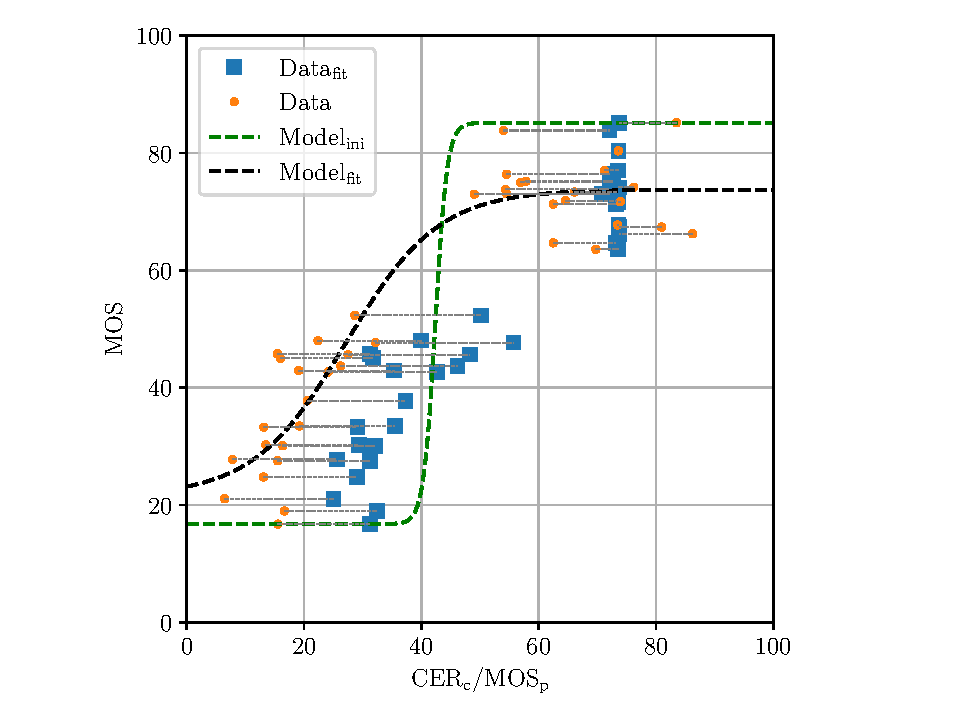
\includegraphics[width=\textwidth]{../exp/fit_example.pdf}
    \caption{Example of the nonlinear fit with subjective and objective values}
    \label{fig:nonlinear_fit}
\end{figure}

In Figure \ref{fig:nonlinear_fit} an example of the nonlinear fit is depicted.
The initial data consists of some randomly generated dummy \gls{mos} and $\text{CER}_{\text{c}}$ values.
The parameters are then adjusted to fit the model to the data.
Finally, we can see that the fitted curve clearly fits the data better than the curve with the initial parameters.
Now the $\text{MOS}_{\text{p}}$ values can be calculated by using the fitted model and the $\text{CER}_{\text{c}}$ values.
With the $\text{MOS}_{\text{p}}$ the three following metrics \cite{iqa_survey_2021} can be calculated.

\section{Pearson Correlation}
\label{sec:pearson}

The \gls{plcc} \cite{pears_spear_2016} describes the linear correlation between two variables, normalized to the range $[-1, 1]$.
Given the $i$th image in our dataset, its \gls{mos} value is denoted as $\text{MOS}_{\text{i}}$ and its predicted \gls{mos} value as $\text{MOS}_{\text{p,i}}$ .
The \gls{plcc} is then defined as follows.

\begin{equation}
    r_{\text{p}} = \frac{\sum_{\text{i}=1}^{N}{(\text{MOS}_{\text{i}}-\overline{\text{MOS}})(\text{MOS}_{\text{i,p}}-\overline{\text{MOS}_{\text{p}}})}}{\sqrt{\sum_{\text{i}=1}^{N}{(\text{MOS}_{\text{i}}-\overline{\text{MOS}})^2}\sum_{\text{i}=1}^{N}{(\text{MOS}_{\text{p,i}}-\overline{\text{MOS}_{\text{p}}})^2}}},
    \label{eq:pearson}
\end{equation}

with $\overline{\text{MOS}}$ and $\overline{\text{MOS}_{\text{p}}}$ representing the mean values of the $\text{MOS}$ and $\text{MOS}_{\text{p}}$ vectors respectively and $N$ the total number of images in the dataset.
$N$ is the total number of images in the images used in the experiment.
If the $r_{\text{p}}$ is close to 1, the two vectors have a positive linear relationship, which means that if $\text{MOS}_{\text{i}}$ increases, $\text{MOS}_{\text{p,i}}$ increases as well.
If the $r_{\text{p}}$ is close to -1, the two vectors have a negative linear relationship, which means that if $\text{MOS}_{\text{i}}$ increases, $\text{MOS}_{\text{p,i}}$ decreases.
If the $r_{\text{p}}$ is close to 0, the two vectors have no correlation at all.
We are using the sample form of the correlations, because we want to make a statement about a much larger population of images, not just our dataset.

\section{Spearman Ranked Correlation}
\label{sec:spearman}

The \gls{srcc} \cite{pears_spear_2016} describes the monotonic correlation between two variables, normalized to the range $[-1, 1]$.
Compared to the \gls{plcc}, it mainly takes the order/rank of the values into account, not the exact values.
The scores $\text{CER}_{\text{c,i}}$ and $\text{MOS}_{\text{i}}$ are transformed into their ranks $\text{CER}_{\text{c,i,r}}$ and $\text{MOS}_{\text{i,r}}$ respectively with values in the range $[1, N]$.
If for example, the first two values are tied, their rank is set to the mean, in this case $(1+2)/2 = 1.5$.
With these values, the \gls{srcc} is defined as follows.

\begin{equation}
    r_{\text{s}} = \frac{\sum_{\text{i}=1}^{N}{(\text{MOS}_{\text{r,i}}-\overline{\text{MOS}_{\text{r}}})(\text{CER}_{\text{c,r,i}}-\overline{\text{CER}_{\text{c,r}}})}}{\sqrt{\sum_{\text{i}=1}^{N}{(\text{MOS}_{\text{r,i}}-\overline{\text{MOS}_{\text{r}}})^2}\sum_{\text{i}=1}^{N}{(\text{CER}_{\text{c,r,i}}-\overline{\text{CER}_{\text{c,r}}})^2}}},
    \label{eq:spearman}
\end{equation}

with $\overline{\text{MOS}_{\text{r}}}$ and $\overline{\text{CER}_{\text{c,r}}}$ representing the mean values of the $\text{MOS}_{\text{r}}$ and $\text{CER}_{\text{c,r}}$ vectors respectively.
If the $r_{\text{s}}$ is close to 1, the two vectors have a positive monotonic relationship, which means that the rank of $\text{CER}_{\text{c,i}}$ increases, while the rank of $\text{MOS}_{\text{i}}$ increases.
If the $r_{\text{s}}$ is close to -1, the two vectors have a negative monotonic relationship, which means that the rank of $\text{CER}_{\text{c,i}}$ increases, while the rank of $\text{MOS}_{\text{i}}$ decreases.
If the $r_{\text{s}}$ is close to 0, the ranks of the two vectors have no correlation at all.
These characteristics will help us to determine if the $\text{CER}_{\text{c}}$ is a good alternative for the \gls{mos}, by checking how similar the ranks of the two metrics are.


\section{Root Mean Squared Error}
\label{sec:rmse}

The \gls{rmse} is a metric that measures the average magnitude of the error between the predicted values and the actual values.
In our case it is defined as follows.

\begin{equation}
    \text{RMSE} = \sqrt{\frac{1}{N}\sum_{i=1}^{N}{(\text{MOS}_{\text{p,i}} - \text{MOS}_{\text{i}})^2}}
    \label{eq:rmse}
\end{equation}

From these metrics, $r_{\text{p}}$ measures the prediction linearity and consistency, $r_{\text{s}}$ measures the prediction monotonicity and the \gls{rmse} measures the prediction accuracy.
With these, we can now determine if the $\text{CER}_{\text{c}}$ is a good alternative for the \gls{mos}.
It is a better alternative the larger $r_s$ and $r_p$ values are, and the smaller the \gls{rmse} is.

Now that we have defined the metrics to evaluate the predicted $\text{CER}_{\text{c}}$ values, the only thing missing is the dataset we use to evaluate the \gls{ocr} algorithms.
Thus in the next chapter we go over what datasets exist and which one we select for our experiments.
